\label{ap:ap06}
\chapter{Arquitetura de dados}
\section*{\textbf{A - ENUNCIADO}}


\subsection*{\textbf{1 Construção de Características: Identificador automático de idioma}}

\textcolor{black}{O problema consiste em criar um modelo de reconhecimento de padrões que dado um texto de entrada, o
programa consegue classificar o texto e indicar a língua em que o texto foi escrito.}



\textcolor{black}{Parta do exemplo (notebook produzido no Colab) que foi disponibilidade e crie as funções para calcular
as diferentes características para o problema da identificação da língua do texto de entrada.}



\textcolor{black}{Nessa atividade é para {\textquotedbl}construir características{\textquotedbl}.}



\textcolor{black}{Meta: a acurácia deverá ser maior ou igual a 70\%.}



\textcolor{black}{Essa tarefa pode ser feita no Colab (Google) ou no Jupiter, em que deverá exportar o notebook e
imprimir o notebook para o formato PDF. Envie no UFPR Virtual os dois arquivos.}



\subsection*{\textbf{2 Melhore uma base de dados ruim}}



\textcolor{black}{Escolha uma base de dados pública para problemas de classificação, disponível ou com origem na UCI
Machine Learning.}



\textcolor{black}{Use o mínimo de intervenção para rodar a SVM e obtenha a matriz de confusão dessa base.}



\textcolor{black}{O trabalho começa aqui, escolha as diferentes tarefas discutidas ao longo da disciplina, para melhorar
essa base de dados, até que consiga efetivamente melhorar o resultado.}



\textcolor{black}{Considerando a acurácia para bases de dados balanceadas ou quase balanceadas, se o percentual da
acurácia original estiver em até 85\%, a meta será obter 5\%. Para bases com mais de 90\% de acurácia, a meta será
obter a melhora em pelo menos 2 pontos percentuais (92\% ou mais).}



\textcolor{black}{Nessa atividade deverá ser entregue o script aplicado (o notebook e o PDF correspondente).}



%%%%%%%%%%%%%%%%%%%%%%%%%%%%%%%%%%%%%%%%%%%%%%%%%%%%%%%%%%%%%%%%%%%%%%%%%%%%%%%%%%%%%%%%%%%%%
\section*{\textbf{B - RESOLUÇÃO}}
\begin{adjustwidth}{1em}{}
\textbf{1 Construção de Características: Identificador automático de idioma}
\end{adjustwidth}

\subsection*{\textbf{Identificador automático de idioma}}
\textbf{Problema:} Dados um texto de entrada, é possível identificar em qual língua o texto está escrito?

Entrada: ``texto qualquer''\\
\indent Saída: português ou inglês ou francês ou italiano ou...

\subsection*{\textbf{O processo de Reconhecimento de Padrões}}
O objetivo desse trabalho é demonstrar o processo de "construção de atributos" e como ele é fundamental para o \textbf{Reconhecimento de Padrões (RP)}.

Primeiro um conjunto de ``amostras'' previamente conhecido (classificado).


\begin{lstlisting}[language=Python, style=input]
#
# amostras de texto em diferentes línguas
#
ingles = [
"Hello, how are you?",
"I love to read books.",
"The weather is nice today.",
"Where is the nearest restaurant?",
"What time is it?",
"I enjoy playing soccer.",
"Can you help me with this?",
"I'm going to the movies tonight.",
"This is a beautiful place.",
"I like listening to music.",
"Do you speak English?",
"What is your favorite color?",
"I'm learning to play the guitar.",
"Have a great day!",
"I need to buy some groceries.",
"Let's go for a walk.",
"How was your weekend?",
"I'm excited for the concert.",
"Could you pass me the salt, please?",
"I have a meeting at 2 PM.",
"I'm planning a vacation.",
"She sings beautifully.",
"The cat is sleeping.",
"I want to learn French.",
"I enjoy going to the beach.",
"Where can I find a taxi?",
"I'm sorry for the inconvenience.",
"I'm studying for my exams.",
"I like to cook dinner at home.",
"Do you have any recommendations for restaurants?",
]

espanhol = [
"Hola, ¿cómo estás?",
"Me encanta leer libros.",
"El clima está agradable hoy.",
"¿Dónde está el restaurante más cercano?",
"¿Qué hora es?",
"Voy al parque todos los días.",
"¿Puedes ayudarme con esto?",
"Me gustaría ir de vacaciones.",
"Este es mi libro favorito.",
"Me gusta bailar salsa.",
"¿Hablas español?",
"¿Cuál es tu comida favorita?",
"Estoy aprendiendo a tocar el piano.",
"Que tengas un buen día!",
"Necesito comprar algunas frutas.",
"Vamos a dar un paseo.",
"¿Cómo estuvo tu fin de semana?",
"Estoy emocionado por el concierto.",
"¿Me pasas la sal, por favor?",
"Tengo una reunión a las 2 PM.",
"Estoy planeando unas vacaciones.",
"Ella canta hermosamente.",
"El perro está jugando.",
"Quiero aprender italiano.",
"Disfruto ir a la playa.",
"¿Dónde puedo encontrar un taxi?",
"Lamento las molestias.",
"Estoy estudiando para mis exámenes.",
"Me gusta cocinar la cena en casa.",
"¿Tienes alguna recomendación de restaurantes?",
]

portugues = [
"Estou indo para o trabalho agora.",
"Adoro passar tempo com minha família.",
"Preciso comprar leite e pão.",
"Vamos ao cinema no sábado.",
"Gosto de praticar esportes ao ar livre.",
"O trânsito está terrível hoje.",
"A comida estava deliciosa!",
"Você já visitou o Rio de Janeiro?",
"Tenho uma reunião importante amanhã.",
"A festa começa às 20h.",
"Estou cansado depois de um longo dia de trabalho.",
"Vamos fazer um churrasco no final de semana.",
"O livro que estou lendo é muito interessante.",
"Estou aprendendo a cozinhar pratos novos.",
"Preciso fazer exercícios físicos regularmente.",
"Vou viajar para o exterior nas férias.",
"Você gosta de dançar?",
"Hoje é meu aniversário!",
"Gosto de ouvir música clássica.",
"Estou estudando para o vestibular.",
"Meu time de futebol favorito ganhou o jogo.",
"Quero aprender a tocar violão.",
"Vamos fazer uma viagem de carro.",
"O parque fica cheio aos finais de semana.",
"O filme que assisti ontem foi ótimo.",
"Preciso resolver esse problema o mais rápido possível.",
"Adoro explorar novos lugares.",
"Vou visitar meus avós no domingo.",
"Estou ansioso para as férias de verão.",
"Gosto de fazer caminhadas na natureza.",
"O restaurante tem uma vista incrível.",
"Vamos sair para jantar no sábado.",
]
\end{lstlisting}

A ``amostras'' de texto precisa ser ``transformada'' em padrões.

Um padrão é um conjunto de características, geralmente representado por um vetor e um conjunto de padrões no formato de tabela. Onde cada linha é um padrão e as colunas as características e, geralmente, na última coluna a classe.


\begin{lstlisting}[language=Python, style=input]
import random

pre_padroes = []
for frase in ingles:
  pre_padroes.append( [frase, 'inglês'])

for frase in espanhol:
  pre_padroes.append( [frase, 'espanhol'])

for frase in portugues:
  pre_padroes.append( [frase, 'português'])

random.shuffle(pre_padroes)

import pandas as pd
dados = pd.DataFrame(pre_padroes)
dados
\end{lstlisting}

\begin{table}[H]
\centering
\begin{tabular}{|c|p{9cm}|c|}
\hline
\textbf{ID} & \textbf{Frase} & \textbf{Idioma} \\
\hline
0 & Me gusta cocinar la cena en casa. & espanhol \\
1 & Vamos fazer uma viagem de carro. & português \\
2 & Do you have any recommendations for restaurants? & inglês \\
3 & Quero aprender a tocar violão. & português \\
4 & Hola, ¿cómo estás? & espanhol \\
\hline
... & ... & ... \\
\hline
87 & Vamos sair para jantar no sábado. & português \\
88 & Estoy emocionado por el concierto. & espanhol \\
89 & Estoy aprendiendo a tocar el piano. & espanhol \\
90 & Preciso fazer exercícios físicos regularmente. & português \\
91 & Quiero aprender italiano. & espanhol \\
\hline
\end{tabular}
\vspace{0.5em}
\caption{Frases com seus respectivos idiomas}
\label{tab:frases_idiomas}
\end{table}


\subsection*{\textbf{Construção dos atributos}}

Esse é o coração desse trabalho e que deverá ser desenvolvido por vocês. Pensem em como podemos "medir" cadas frase/sentença e extrair características que melhorem o resultado do processo de identificação.


Após a criação de cada novo atributo, execute as etapas seguintes e registre as métricas da matriz de confusão. Principalmente acurácia e a precisão.


\begin{lstlisting}[language=Python, style=input]
# a entrada é o vetor pre_padroes e a saída desse passo deverá ser "padrões"
import re
from sklearn.feature_extraction.text import CountVectorizer

def tamanhoMedioFrases(texto):
  palavras = re.split("\s",texto)
  #print(palavras)
  tamanhos = [len(s) for s in palavras if len(s)>0]
  #print(tamanhos)
  soma = 0
  for t in tamanhos:
    soma=soma+t
  return soma / len(tamanhos)

def temCaractere(texto, simbolo):
  return int(simbolo in texto)

def gerarNGrams(list_textos, n, max_f):
  vec = CountVectorizer(analyzer='char', ngram_range=(n,n), max_features=max_f)
  ngrams = vec.fit_transform(list_textos)
  feature_names = vec.get_feature_names_out()

  return feature_names

def extraiCaracteristicas(frase):
  # frase é um vetor [ 'texto', 'lingua' ]
  texto = frase[0]
  pattern_regex = re.compile('[^\w+]', re.UNICODE)
  texto = re.sub(pattern_regex,' ',texto)
  #print(texto)
  caracteristica1=tamanhoMedioFrases(texto)

  #ESTRATEGIA 1: buscando caracteres especiais
  caracteristica2=temCaractere(texto, 'ç')
  caracteristica3=temCaractere(texto, 'ñ')
  caracteristica12=temCaractere(texto, 'à')
  caracteristica13=temCaractere(texto, 'ón')
  caracteristica14=temCaractere(texto, 'ã')
  caracteristica15=temCaractere(texto, 'ay')
  caracteristica16=temCaractere(texto, 'yo')

  #ESTRATEGIA 2: buscando caracteres iguais sucessivos
  caracteristica4=temCaractere(texto, 'cc')
  caracteristica5=temCaractere(texto, 'oo')
  caracteristica6=temCaractere(texto, 'll')
  caracteristica7=temCaractere(texto, 'ss')
  caracteristica8=temCaractere(texto, 'mm')
  caracteristica9=temCaractere(texto, 'nn')
  caracteristica10=temCaractere(texto, 'rr')
  caracteristica11=temCaractere(texto, 'ee')

  #ESTRATEGIA 3: buscando ocorrencia dos ngrams mais frequentes por lingua
  features_ngrams = []

  for n in ngrams_populares_p_lingua:
    features_ngrams.append(int(n in texto))

  # acrescente as suas funcoes no vetor padrao
  padrao = [caracteristica1, caracteristica2, caracteristica3,
            caracteristica4, caracteristica5, caracteristica6,
            caracteristica7, caracteristica8, caracteristica9,
            caracteristica10, caracteristica11,
            caracteristica12, caracteristica13, caracteristica14, caracteristica15, caracteristica16,
            *features_ngrams,
            frase[1]]

  return padrao


def geraPadroes(frases):
  padroes = []
  for frase in frases:
    padrao = extraiCaracteristicas(frase)
    padroes.append(padrao)
  return padroes

#GERA 88 1,2,3,4-GRAMS MAIS COMUNS PARA CADA LINGUA
#set para evitar repetidos
ngrams_populares_p_lingua = set()
max_features = 38 # ou 88
for nsize in range(1, 5): # ou 4
  ngrams_populares_p_lingua.update(gerarNGrams(portugues, nsize, max_features))
  ngrams_populares_p_lingua.update(gerarNGrams(ingles, nsize, max_features))
  ngrams_populares_p_lingua.update(gerarNGrams(espanhol, nsize, max_features))

# converte o formato [frase classe] em
# [caracteristica_1, caracteristica_2,... caracteristica n, classe]
padroes = geraPadroes(pre_padroes)

#
# apenas para visualizacao
print(padroes)

dados = pd.DataFrame(data=padroes, columns=['TMediaFrase','ç','ñ','cc','oo','ll','ss','mm','nn','rr','ee', 'à', 'ón', 'ã', 'ay', 'yo', *ngrams_populares_p_lingua, 'Lingua'])
dados
\end{lstlisting}


\subsection*{\textbf{Treinando o modelo com SVM}}

Separando o conjunto de treinamento do conjunto de testes


\begin{lstlisting}[language=Python, style=input]
from sklearn.model_selection import train_test_split
import numpy as np


#from sklearn.metrics import confusion_matrix

vet = np.array(padroes)
classes = vet[:,-1]         # classes = [p[-1] for p in padroes]
#print(classes)
padroes_sem_classe = vet[:,0:-1]
#print(padroes_sem_classe)
X_train, X_test, y_train, y_test = train_test_split(padroes_sem_classe, classes, test_size=0.20, stratify=classes)
\end{lstlisting}

Com os conjuntos separados, podemos "treinar" o modelo usando a SVM.

\begin{lstlisting}[language=Python, style=input]
  from sklearn import svm
from sklearn.metrics import confusion_matrix
from sklearn.metrics import classification_report

treinador = svm.SVC()  #algoritmo escolhido
modelo = treinador.fit(X_train, y_train)

#
# score com os dados de treinamento
acuracia = modelo.score(X_train, y_train)
print("Acurácia nos dados de treinamento: {:.2f}%".format(acuracia * 100))

#
# melhor avaliar com a matriz de confusão
y_pred = modelo.predict(X_train)
cm = confusion_matrix(y_train, y_pred)
print(cm)
print(classification_report(y_train, y_pred))

#
# com dados de teste que não foram usados no treinamento
print('métricas mais confiáveis')
y_pred2 = modelo.predict(X_test)
cm = confusion_matrix(y_test, y_pred2)
print(cm)
print(classification_report(y_test, y_pred2))
\end{lstlisting}


\begin{lstlisting}[language=, style=output]
Acuracia nos dados de treinamento: 98.63%
[[24  0  0]
 [ 0 24  0]
 [ 1  0 24]]
              precision    recall  f1-score   support

    espanhol       0.96      1.00      0.98        24
      ingles       1.00      1.00      1.00        24
   portugues       1.00      0.96      0.98        25

    accuracy                           0.99        73
   macro avg       0.99      0.99      0.99        73
weighted avg       0.99      0.99      0.99        73

metricas mais confiaveis
[[6 0 0]
 [0 5 1]
 [4 0 3]]
              precision    recall  f1-score   support

    espanhol       0.60      1.00      0.75         6
      ingles       1.00      0.83      0.91         6
   portugues       0.75      0.43      0.55         7

    accuracy                           0.74        19
   macro avg       0.78      0.75      0.73        19
weighted avg       0.78      0.74      0.72        19
\end{lstlisting}


\begin{adjustwidth}{1em}{}
\textbf{2 Melhore uma base de dados ruim}
\end{adjustwidth}


\begin{lstlisting}[language=Python, style=input]
import numpy as np
import pandas as pd

from sklearn.model_selection import train_test_split
from sklearn import svm
from sklearn.metrics import confusion_matrix
from sklearn.metrics import classification_report
from sklearn.preprocessing import scale
from sklearn.preprocessing import minmax_scale
from sklearn.preprocessing import StandardScaler

df = pd.read_csv('heart_failure_clinical_records_dataset.csv')
df.describe()
\end{lstlisting}

\begin{table}[H]
\centering
\begin{adjustbox}{width=\textwidth}
\begin{tabular}{|l|rrrrrrr|}
\hline
\textbf{Stat} & \textbf{age} & \textbf{anaemia} & \textbf{creatinine\_phosphokinase} & \textbf{diabetes} & \textbf{ejection\_fraction} & \textbf{high\_blood\_pressure} & \textbf{platelets} \\
\hline
count & 299.000 & 299.000 & 299.000 & 299.000 & 299.000 & 299.000 & 299.000 \\
mean & 60.834 & 0.431 & 581.839 & 0.418 & 38.084 & 0.351 & 263358.029 \\
std & 11.895 & 0.496 & 970.288 & 0.494 & 11.835 & 0.478 & 97804.237 \\
min & 40.000 & 0.000 & 23.000 & 0.000 & 14.000 & 0.000 & 25100.000 \\
25\% & 51.000 & 0.000 & 116.500 & 0.000 & 30.000 & 0.000 & 212500.000 \\
50\% & 60.000 & 0.000 & 250.000 & 0.000 & 38.000 & 0.000 & 262000.000 \\
75\% & 70.000 & 1.000 & 582.000 & 1.000 & 45.000 & 1.000 & 303500.000 \\
max & 95.000 & 1.000 & 7861.000 & 1.000 & 80.000 & 1.000 & 850000.000 \\
\hline
\end{tabular}
\end{adjustbox}
%\caption{Descriptive statistics (Part 1)}
\label{tab:heart_stats_part1}
\end{table}

\begin{table}[H]
\centering
\begin{adjustbox}{width=\textwidth}
\begin{tabular}{|l|rrrrrr|}
\hline
\textbf{Stat} & \textbf{serum\_creatinine} & \textbf{serum\_sodium} & \textbf{sex} & \textbf{smoking} & \textbf{time} & \textbf{DEATH\_EVENT} \\
\hline
count & 299.000 & 299.000 & 299.000 & 299.000 & 299.000 & 299.000 \\
mean & 1.394 & 136.625 & 0.649 & 0.321 & 130.261 & 0.321 \\
std & 1.035 & 4.412 & 0.478 & 0.468 & 77.614 & 0.468 \\
min & 0.500 & 113.000 & 0.000 & 0.000 & 4.000 & 0.000 \\
25\% & 0.900 & 134.000 & 0.000 & 0.000 & 73.000 & 0.000 \\
50\% & 1.100 & 137.000 & 1.000 & 0.000 & 115.000 & 0.000 \\
75\% & 1.400 & 140.000 & 1.000 & 1.000 & 203.000 & 1.000 \\
max & 9.400 & 148.000 & 1.000 & 1.000 & 285.000 & 1.000 \\
\hline
\end{tabular}
\end{adjustbox}
%\caption{Descriptive statistics (Part 2)}
\label{tab:heart_stats_part2}
\end{table}


\begin{lstlisting}[language=Python, style=input]
import seaborn as sns
corr = df.corr()
sns.heatmap(corr,
            xticklabels=corr.columns.values,
            yticklabels=corr.columns.values)
\end{lstlisting}

\begin{figure}[H]
\centering
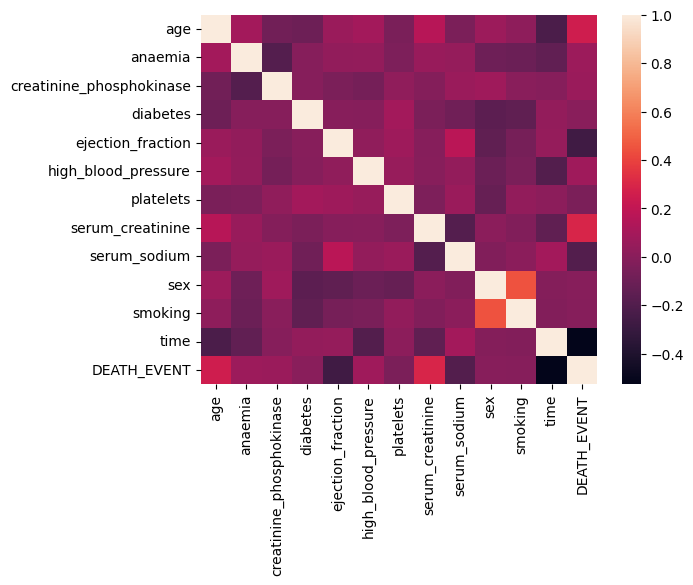
\includegraphics[width=1\linewidth]{apendices/fig/6_IAA006_1.png}
\caption{Mapa de correlação dados clínicos}
\end{figure}


\begin{lstlisting}[language=Python, style=input]
X_orig = df.iloc[:,:-1]
y_orig = df['DEATH_EVENT']

X_train_orig, X_test_orig, y_train, y_test = train_test_split(X_orig, y_orig, test_size=0.20, stratify=y_orig,random_state=10)

treinador = svm.SVC()  #algoritmo escolhido

modelo_orig = treinador.fit(X_train_orig, y_train)

# predição com os mesmos dados usados para treinar
y_pred = modelo_orig.predict(X_train_orig)
cm_orig_train = confusion_matrix(y_train, y_pred)
print('Matriz de confusao - com os dados ORIGINAIS usados no TREINAMENTO')
#print(cm_orig_train)
print(classification_report(y_train, y_pred, zero_division=0))

# predição com os mesmos dados usados para testar
y2_pred = modelo_orig.predict(X_test_orig)
cm_orig_test = confusion_matrix(y_test, y2_pred)
print('Matriz de confusao - com os dados ORIGINAIS usados para TESTES')
#print(cm_orig_test)
print(classification_report(y_test, y2_pred, zero_division=0))
\end{lstlisting}


\begin{lstlisting}[language=, style=output]
Matriz de confusao - com os dados ORIGINAIS usados no TREINAMENTO
              precision    recall  f1-score   support

           0       0.68      1.00      0.81       162
           1       0.00      0.00      0.00        77

    accuracy                           0.68       239
   macro avg       0.34      0.50      0.40       239
weighted avg       0.46      0.68      0.55       239

Matriz de confusao - com os dados ORIGINAIS usados para TESTES
              precision    recall  f1-score   support

           0       0.68      1.00      0.81        41
           1       0.00      0.00      0.00        19

    accuracy                           0.68        60
   macro avg       0.34      0.50      0.41        60
weighted avg       0.47      0.68      0.55        60
\end{lstlisting}


\begin{lstlisting}[language=Python, style=input]
y = df['DEATH_EVENT']
X = df.drop(['diabetes', 'time', 'DEATH_EVENT'],axis = 1)

X_train, X_test, y_train, y_test = train_test_split(X, y, test_size=0.20, stratify=y_orig,random_state=10)

scaler = StandardScaler().fit(X_train)
X_train_scaled = scaler.transform(X_train)
X_test_scaled = scaler.transform(X_test)

treinador = svm.SVC()  #algoritmo escolhido

modelo_orig = treinador.fit(X_train_scaled, y_train)

# predição com os mesmos dados usados para treinar
y_pred = modelo_orig.predict(X_train_scaled)
cm_orig_train = confusion_matrix(y_train, y_pred)
print('Matriz de confusao - com os dados escalonados e de alta correlacao usados no TREINAMENTO')
#print(cm_orig_train)
print(classification_report(y_train, y_pred, ))

# predição com os mesmos dados usados para testar
y2_pred = modelo_orig.predict(X_test_scaled)
cm_orig_test = confusion_matrix(y_test, y2_pred)
print('Matriz de confusao - com os dados escalonados e de alta correlacao usados no TESTE')
#print(cm_orig_test)
print(classification_report(y_test, y2_pred))
\end{lstlisting}


\begin{lstlisting}[language=, style=output]
Matriz de confusao - com os dados escalonados e de alta correlacao usados no TREINAMENTO
              precision    recall  f1-score   support

           0       0.83      0.96      0.89       162
           1       0.88      0.60      0.71        77

    accuracy                           0.85       239
   macro avg       0.86      0.78      0.80       239
weighted avg       0.85      0.85      0.84       239

Matriz de confusao - com os dados escalonados e de alta correlacao usados no TESTE
              precision    recall  f1-score   support

           0       0.78      0.85      0.81        41
           1       0.60      0.47      0.53        19

    accuracy                           0.73        60
   macro avg       0.69      0.66      0.67        60
weighted avg       0.72      0.73      0.72        60
\end{lstlisting}